\chapter{Results}\label{Sec:Results}

\section{Maximal Representative Subsample}
 
There is almost always not enough data available to partition it into separate training and test sets without losing significant modelling or testing capability. In these cases, a fair way to properly estimate model prediction performance is to use cross-validation as a powerful general technique[5].

The overly optimistic resubstitution error, is not a good indicator of model performance. To evaluate the actual performance of a model, the given data samples need to be split. The proper procedure uses three sets: training data, validation data, and test data [2]. The holdout method is the most common approach to get a reliable performance estimation: A certain amount of data is reserved for testing while the remainder is used for the actual training. Because the method is very fast, it is useful to use when the algorithm is slow to train and the dataset is large. Training and test sets might not be representative of the same underlying distribution, e.g. class hardly represented in the test set.

The holdout estimate can be made more reliable by repeating the process with different subsamples. The error rates on the different iterations are averaged to yield an overall error rate. To further reduce the variance of the error estimate, each class is sampled with approximately equal proportions in both datasets, a technique called stratification. Figure X shows the results on the GFI-10 data.

\subsection{Fraction of Positives}

Estimating Positive Class Prior with One-Class SVMs. Using the One-Class SVM and its ability to capture the shape of the data set, hence performing better when the data is strongly non-Gaussian, i.e. with two well-separated clusters;

\begin{figure}[ht]
	\begin{center}
		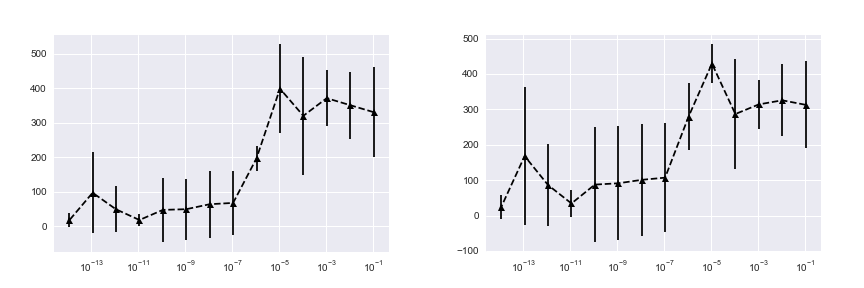
\includegraphics[scale=0.55,angle=0]{fig/occfigure}
		\label{occ}
		\vspace*{-1.0cm}
		\caption{Tuning parameter \(nu\) that controls the trade-off between the fraction of non-representative samples and the number of support vectors in one-class SVM. More than 0.73 of GBS (right) are classified as representative with high confidence (low sdt) for the optimal value \(nu = 10^{-5}\).}
	\end{center}
\end{figure}

\subsection{ROC and puROC Evaluation}

\begin{figure}
\centering
		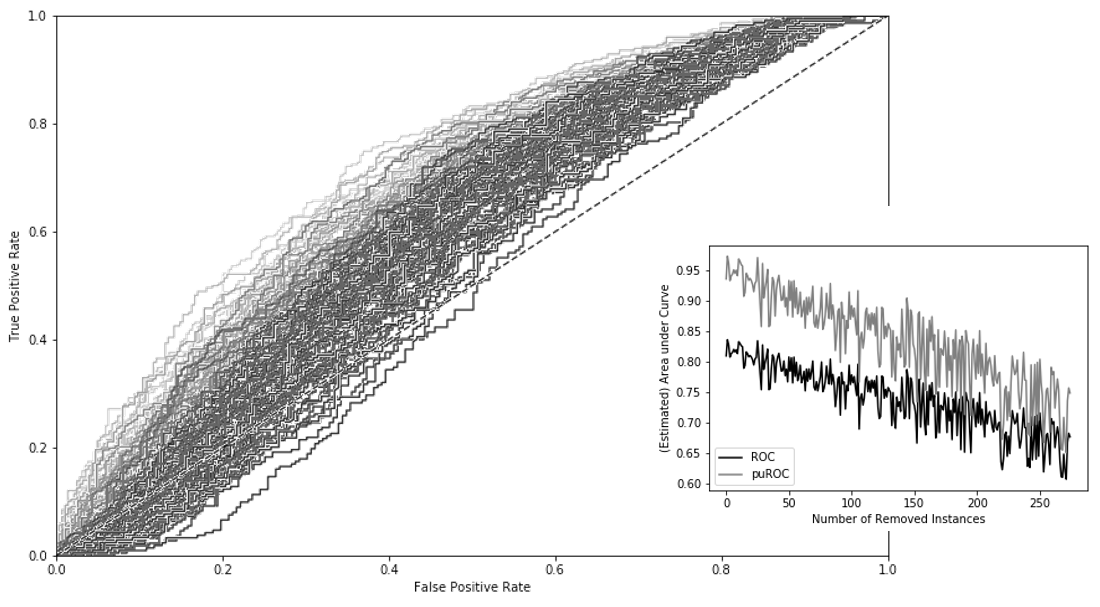
\includegraphics[scale=0.50,angle=0]{fig/res1}
   \label{fig:Ng1} 
\end{figure}

\section{Political Participation and Resilience}

In modelling a political participation process, a computer program is designed to approximate the likelihood of a person going to vote on election day. Ideally, for every instance with unknown political interest and willingness to participate, there is enough data of people of similiar demographics, socioeconomics and psychological traits to generalize from. 

\begin{figure}
\centering
\begin{subfigure}[b]{0.8\textwidth}
		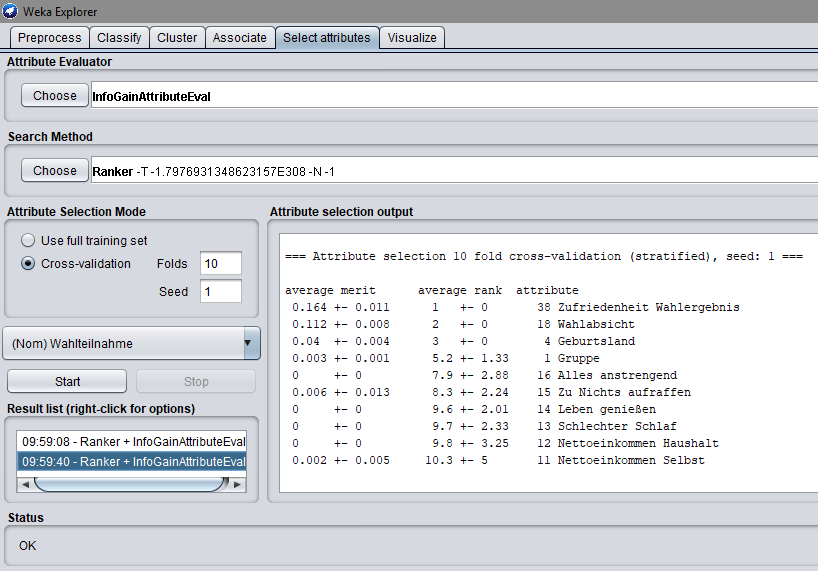
\includegraphics[scale=0.55,angle=0]{fig/weka_gbs}
   \label{fig:Ng1} 
\end{subfigure}

\begin{subfigure}[b]{0.8\textwidth}
\vspace{0.55cm}
		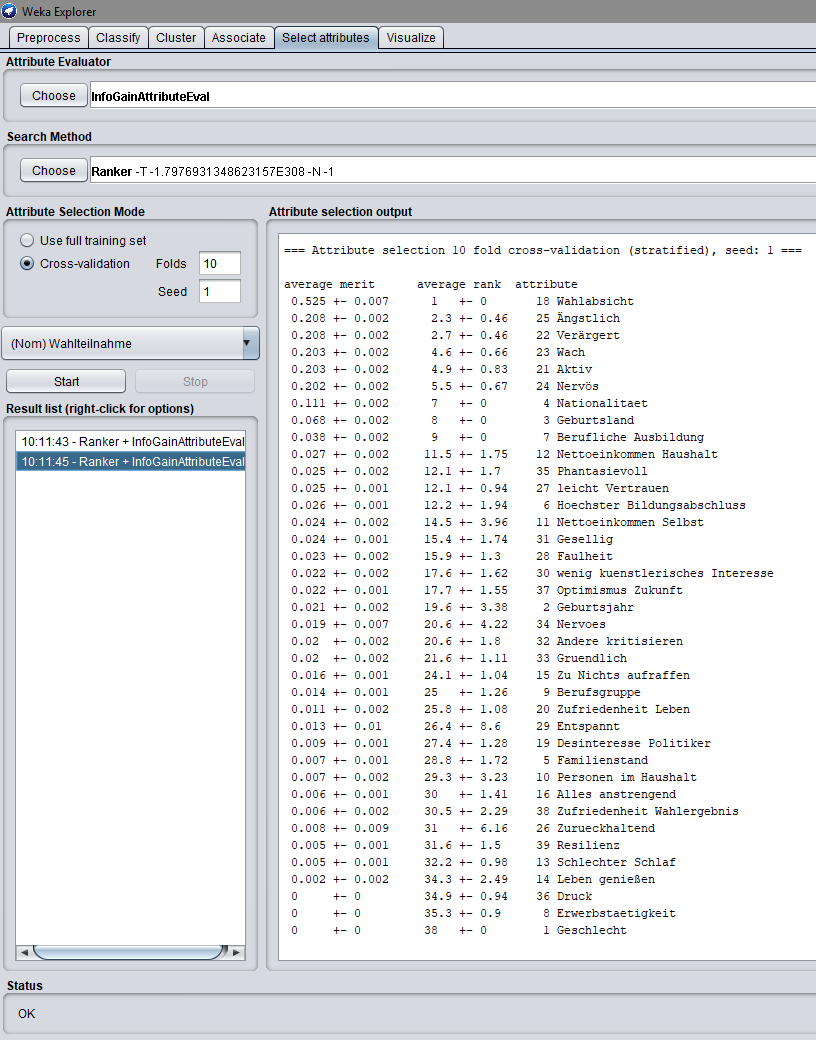
\includegraphics[scale=0.55,angle=0]{fig/weka_gesis}
   \label{fig:Ng2}
\end{subfigure}
\vspace{0.35cm}
\caption{Feature importance GBS (n=579) and GBS MRS (n=280) in classification of political participation "Wahlteilnahme".}
\end{figure}

